\chapter{التفاعلات الكيميائية: المتفاعلات والنواتج}\label{ch:g7:chemical-reactions}

يتوهج الفحم في الشواية. وبعد ساعة لا يكاد يبقى شيء من الكتل السوداء ---
قليل من الرماد الرمادي، والحرارة التي أنضجت الطعام. فأين ذهب الكربون
الأسود؟ لم يتلاشَ: بل التقى أكسجين \omterm{def:g4:air-a-mixture-of-gases:air}{الهواء} وصار غازًا جديدًا لا يُرى.
وبعد أن عرفنا \omterm{def:g7:atoms-and-molecules:atom}{الذرات} \omterm{def:g7:atoms-and-molecules:molecule}{والجزيئات} نستطيع الآن أن نقول بدقة ماذا يحدث في
مثل هذا التغير.

\begin{recall}
في \omterm{def:g5:irreversible-changes:chemical-change}{التغير الكيميائي} تظهر مواد جديدة ولا توجد طريق بسيطة للعودة
(\cref{ch:g5:irreversible-changes}). وماء الجير يتعكّر بثنائي أكسيد
الكربون، وكبريتات النحاس اللامائية تزرقّ بالماء
(\cref{ch:g7:identifying-substances}). وكل المادة مكوّنة من \omterm{def:g7:atoms-and-molecules:atom}{ذرات} تتجمع
في \omterm{def:g7:atoms-and-molecules:molecule}{جزيئات}؛ والصيغة مثل \ce{CO2} تذكر \omterm{def:g7:atoms-and-molecules:atom}{ذرات}
\omterm{def:g7:atoms-and-molecules:molecule}{الجزيء} (\cref{ch:g7:atoms-and-molecules}).
\end{recall}

\begin{omfigure}
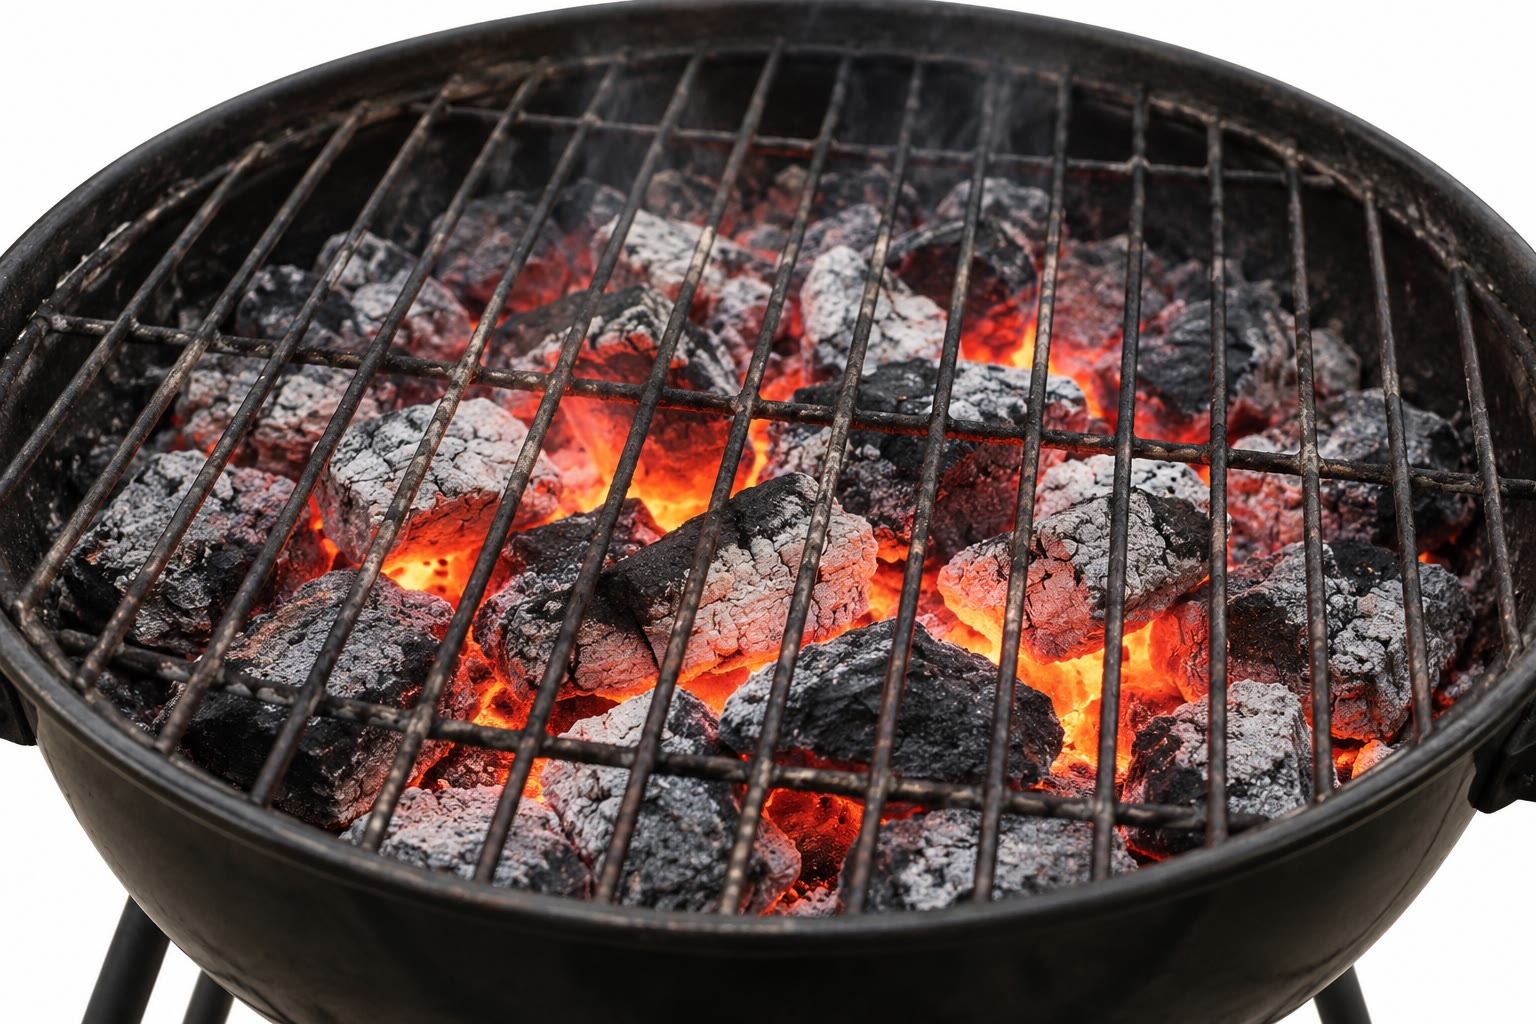
\includegraphics[width=0.55\linewidth]{images/book1/ai/g7-charcoal-bbq.jpg}

{\small فحم متوهج: كربون يتفاعل مع أكسجين \omterm{def:g4:air-a-mixture-of-gases:air}{الهواء}.}
\end{omfigure}

\section{التحولات الفيزيائية والتحولات الكيميائية}

\begin{definition}[التحول الفيزيائي]\label{def:g7:chemical-reactions:physical-transformation}
\emph{التحول الفيزيائي}\index{تحول فيزيائي} يغيّر حالة المادة أو ترتيبها
دون أن يغيّر الأنواع الكيميائية: الانصهار، والتجمد، والغليان، \omterm{def:g2:mixing-and-dissolving:dissolve}{والذوبان}،
\omterm{def:g2:mixing-and-dissolving:mix}{والخلط}. فالأنواع نفسها موجودة قبله وبعده؛ ولم يتغير إلا شكلها أو
ترتيبها.
\end{definition}

\begin{example}[الماء بثلاث طرائق]\label{ex:g7:chemical-reactions:water}
انصهار الجليد ماءً، وغليان الماء بخارًا، \omterm{def:g2:mixing-and-dissolving:dissolve}{وذوبان} الملح في الماء تحولات
فيزيائية: فقبلها وبعدها توجد \omterm{def:g7:atoms-and-molecules:molecule}{جزيئات} الماء (والملح). وإذا كبّرنا الصورة
وجدنا \omterm{def:g7:atoms-and-molecules:molecule}{الجزيئات} نفسها؛ ولم يتغير إلا ترتيبها وطريقة حركتها.
\end{example}

\begin{proposition}[التحول الكيميائي]\label{prop:g7:chemical-reactions:chemical}
في \omterm{def:g5:irreversible-changes:chemical-change}{التغير الكيميائي}، ويسمى أيضًا التحول الكيميائي، تختفي بعض الأنواع
الكيميائية وتظهر أنواع جديدة. ويُميَّز من \omterm{def:g7:chemical-reactions:physical-transformation}{التحول الفيزيائي} بنواتجه: أنواع
جديدة يمكن الكشف عنها باختبارات مميِّزة.
\end{proposition}

\begin{omfigure}
\begin{tikzpicture}[font=\small, level distance=1.5cm,
    box/.style={draw=omDef, fill=omDef!6, rounded corners=2pt, align=center,
      inner sep=4pt},
    level 1/.style={sibling distance=6.6cm},
    edge from parent/.style={draw, thick, omDef, ->}]
  \node[box] {تحول للمادة}
    child {node[box, text width=5.2cm] {\textbf{فيزيائي}: الأنواع نفسها\\
        قبله وبعده\\ \footnotesize الانصهار، الغليان، الذوبان}}
    child {node[box, draw=omProp, fill=omProp!6, text width=5.2cm]
      {\textbf{كيميائي}: تختفي أنواع،\\ وتظهر أنواع جديدة\\
        \footnotesize الاحتراق، الصدأ، الطهو}};
\end{tikzpicture}

{\small نوعان من التحولات.}
\end{omfigure}

\section{المتفاعلات والنواتج}

\begin{definition}[التفاعل الكيميائي]\label{def:g7:chemical-reactions:reaction}
\emph{التفاعل الكيميائي}\index{تفاعل كيميائي} هو النموذج الذي يستعمله
الكيميائيون لوصف التحول الكيميائي: فهو يذكر الأنواع التي تُستهلك والأنواع
التي تتكوّن.
\end{definition}

\begin{definition}[المتفاعلات والنواتج]\label{def:g7:chemical-reactions:reactant}
الأنواع التي تُستهلك في \omterm{def:g7:chemical-reactions:reaction}{التفاعل الكيميائي} هي
\emph{المتفاعلات}\index{متفاعل}؛ والأنواع التي تتكوّن هي
\emph{النواتج}\index{ناتج}.
\end{definition}

\begin{example}[احتراق الكربون في الأكسجين]\label{ex:g7:chemical-reactions:carbon}
حين يحترق الفحم تكون \omterm{def:g7:chemical-reactions:reactant}{المتفاعلات} هي الكربون (الفحم) والأكسجين (من
\omterm{def:g4:air-a-mixture-of-gases:air}{الهواء}). \omterm{def:g7:chemical-reactions:reactant}{والناتج} هو ثنائي أكسيد الكربون: فإذا رُجّ الغاز الباقي في المخبار مع
ماء الجير عكّره.
\end{example}

\begin{inthelab}[الفحم في مخبار من الأكسجين]
يسخّن المعلم قطعة صغيرة من الفحم على ملعقة \omterm{def:g4:what-a-fire-needs:burning}{احتراق} حتى تتوهج، ثم يُنزلها
في مخبار مملوء بالأكسجين. فيتوهج الفحم أشد بكثير مما في \omterm{def:g4:air-a-mixture-of-gases:air}{الهواء} ويصغر حتى
يختفي. ثم يُغطى المخبار، ويُصب فيه قليل من ماء الجير ويُرج: فيتعكّر.
لقد استُهلك الكربون والأكسجين؛ وتكوّن ثنائي أكسيد الكربون.
\end{inthelab}

\begin{omfigure}
\begin{tikzpicture}[font=\small, scale=1.3]
  \pic[transform shape] at (0,0) {gasjaropen={0}{white}};
  \fill[omWater!60] (-0.68,2.62) rectangle (0.68,2.7);
  \draw[omGlass, line width=0.4pt] (-0.68,2.62) rectangle (0.68,2.7);
  \draw[black!60, line width=1.2pt] (0.15,2.7) -- (0.15,3.6) -- (1.2,3.6);
  \draw[black!60, line width=1.2pt] (0.15,2.7) -- (0.15,1.2);
  \fill[black!60] (-0.12,1.12) rectangle (0.32,1.2);
  \fill[red!70!black] (0.0,1.32) circle (0.13);
  \fill[orange!90!yellow] (0.0,1.32) circle (0.08);
  \draw[<-, omProp, thick] (0.15,1.35) -- (1.5,1.6) node[right, text=black]
    {فحم متوهج (كربون)};
  \draw[<-, omProp, thick] (-0.35,2.1) -- (1.5,2.3) node[right, text=black]
    {أكسجين};
  \draw[<-, omProp, thick] (0.6,2.66) -- (1.5,2.95) node[right, text=black]
    {غطاء};
  \draw[<-, omProp, thick] (0.15,3.1) -- (1.5,3.6) node[right, text=black]
    {ملعقة احتراق};
\end{tikzpicture}

{\small الفحم المتوهج الذي يُنزل على ملعقة في مخبار من الأكسجين يحترق
بشدة: يتفاعل الكربون والأكسجين فيتكوّن ثنائي أكسيد الكربون.}
\end{omfigure}

\begin{example}[الصوف الفولاذي]\label{ex:g7:chemical-reactions:steel-wool}
يمكن لوسادة من الصوف الفولاذي الدقيق، وهو في معظمه حديد، أن تحترق في
\omterm{def:g4:air-a-mixture-of-gases:air}{الهواء} مع وابل من الشرر. \omterm{def:g7:chemical-reactions:reactant}{المتفاعلات} هي الحديد والأكسجين؛ \omterm{def:g7:chemical-reactions:reactant}{والناتج} جسم صلب
داكن هشّ، هو أكسيد للحديد.
\end{example}

\begin{omfigure}
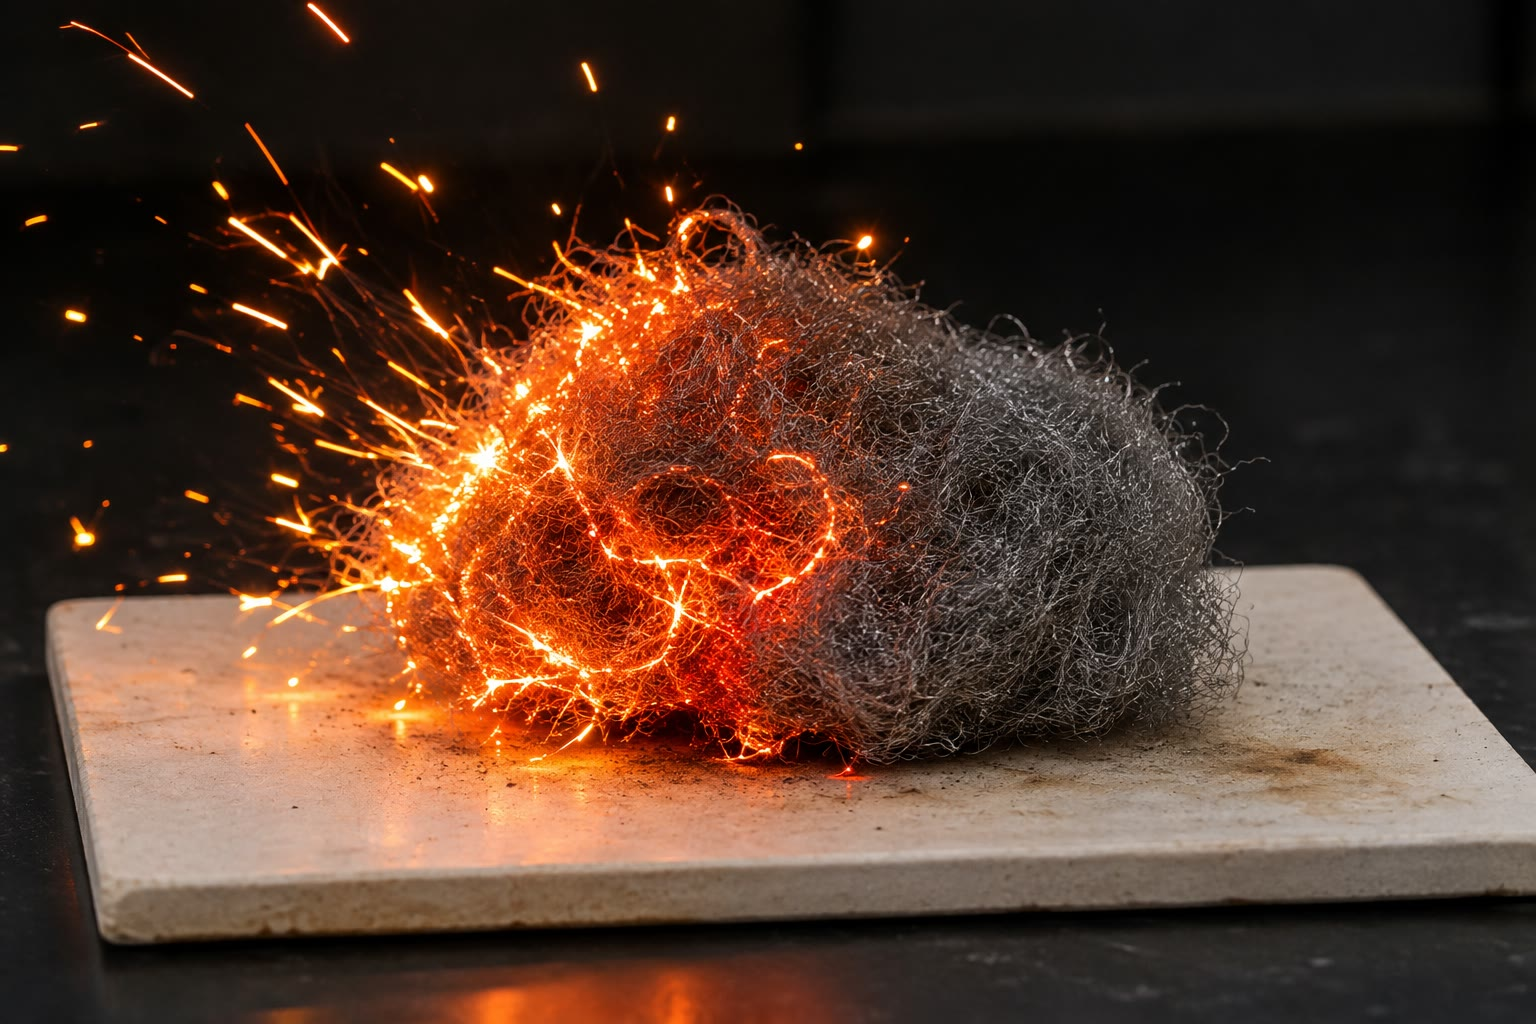
\includegraphics[width=0.5\linewidth]{images/book1/ai/g7-steel-wool-burning.jpg}

{\small صوف فولاذي يحترق في المختبر: يتفاعل الحديد والأكسجين.}
\end{omfigure}

\section{المعادلة اللفظية}

\begin{definition}[المعادلة اللفظية]\label{def:g7:chemical-reactions:word-equation}
\emph{المعادلة اللفظية}\index{معادلة لفظية} تكتب \omterm{def:g7:chemical-reactions:reaction}{التفاعل الكيميائي}
بالكلمات: أسماء \omterm{def:g7:chemical-reactions:reactant}{المتفاعلات} على اليمين، يربط بينها $+$، ثم سهم، ثم
أسماء \omterm{def:g7:chemical-reactions:reactant}{النواتج} على اليسار. ويُقرأ السهم «تتفاعل
فتعطي».
\end{definition}

\begin{example}[ثلاث معادلات لفظية]\label{ex:g7:chemical-reactions:three}
\begin{center}
\begin{tabular}{l}
كربون $+$ أكسجين $\longleftarrow$ ثنائي أكسيد الكربون\\[2pt]
ميثان $+$ أكسجين $\longleftarrow$ ثنائي أكسيد الكربون $+$ ماء\\[2pt]
حديد $+$ أكسجين $\longleftarrow$ أكسيد الحديد
\end{tabular}
\end{center}
\end{example}

\begin{method}[كتابة المعادلة اللفظية]\label{met:g7:chemical-reactions:write}
\begin{enumerate}
  \item جد \omterm{def:g7:chemical-reactions:reactant}{المتفاعلات}: الأنواع التي تختفي.
  \item جد \omterm{def:g7:chemical-reactions:reactant}{النواتج}: الأنواع الجديدة التي تُعرف بالاختبارات.
  \item اكتب \omterm{def:g7:chemical-reactions:reactant}{المتفاعلات} على اليمين \omterm{def:g7:chemical-reactions:reactant}{والنواتج} على اليسار، وبينها
        سهم؛ ولا تكتب أبدًا علامة التساوي.
\end{enumerate}
والنوع الموجود الذي لا يشارك في التفاعل --- مثل نيتروجين \omterm{def:g4:air-a-mixture-of-gases:air}{الهواء}
المحيط باللهب --- لا يُكتب.
\end{method}

\section{التفاعل إعادة ترتيب للذرات}

\begin{proposition}[يُعاد ترتيب الذرات]\label{prop:g7:chemical-reactions:rearranged}
في \omterm{def:g7:chemical-reactions:reaction}{التفاعل الكيميائي} تتفكك \omterm{def:g7:atoms-and-molecules:molecule}{جزيئات} \omterm{def:g7:chemical-reactions:reactant}{المتفاعلات}، وتتحد ذراتها على نحو مختلف
لتبني \omterm{def:g7:atoms-and-molecules:molecule}{جزيئات} \omterm{def:g7:chemical-reactions:reactant}{النواتج}. \omterm{def:g7:atoms-and-molecules:atom}{والذرات} نفسها لا تُخلق ولا تفنى: \omterm{def:g7:atoms-and-molecules:atom}{فالذرات} نفسها،
بالأعداد نفسها، موجودة قبل التفاعل وبعده.
\end{proposition}

\begin{example}[احتراق الميثان جزيئًا جزيئًا]\label{ex:g7:chemical-reactions:methane}
حين يحترق ميثان موقد الغاز يلتقي \omterm{def:g7:atoms-and-molecules:molecule}{جزيء} ميثان واحد \ce{CH4} بجزيئي
أكسجين \ce{O2}. فيُعاد ترتيب ذراتها في \omterm{def:g7:atoms-and-molecules:molecule}{جزيء} واحد من ثنائي أكسيد الكربون
\ce{CO2} وجزيئي ماء \ce{H2O}. قبل: \omterm{def:g7:atoms-and-molecules:atom}{ذرة} كربون واحدة، و4 \omterm{def:g7:atoms-and-molecules:atom}{ذرات}
هيدروجين، و4 \omterm{def:g7:atoms-and-molecules:atom}{ذرات} أكسجين. وبعد: \omterm{def:g7:atoms-and-molecules:atom}{ذرة} كربون واحدة، و4 \omterm{def:g7:atoms-and-molecules:atom}{ذرات} هيدروجين،
و$2 + 2 = 4$ \omterm{def:g7:atoms-and-molecules:atom}{ذرات} أكسجين. فلا يضيع شيء، ولا يظهر شيء من
العدم.
\end{example}

\begin{omfigure}
\begin{tikzpicture}[font=\small]
  % methane
  \begin{scope}[xshift=0cm]
    \node[aC] (c) at (0,0) {};
    \node[aH] (h1) at (0,0.78) {}; \node[aH] (h2) at (-0.74,-0.3) {};
    \node[aH] (h3) at (0.74,-0.3) {}; \node[aH] (h4) at (0.2,-0.68) {};
    \begin{scope}[on background layer]
      \foreach \h in {h1,h2,h3,h4} \draw[bond] (c.center) -- (\h.center);
    \end{scope}
    \node at (0,-1.2) {\foreignlanguage{arabic}{\babelsublr{1} ميثان}};
  \end{scope}
  \node at (1.45,0) {$+$};
  % two oxygen molecules
  \foreach \y in {0.45,-0.45} {
    \node[aO] (a) at (2.4,\y) {}; \node[aO] (b) at (3.05,\y) {};
    \begin{scope}[on background layer]
      \draw[bond, line width=1.1pt] ([yshift=1.6pt]a.center) -- ([yshift=1.6pt]b.center);
      \draw[bond, line width=1.1pt] ([yshift=-1.6pt]a.center) -- ([yshift=-1.6pt]b.center);
    \end{scope}
  }
  \node at (2.72,-1.2) {\foreignlanguage{arabic}{\babelsublr{2} أكسجين}};
  \draw[->, thick, omProp] (3.8,0) -- (5.0,0);
  % carbon dioxide
  \begin{scope}[xshift=6.3cm]
    \node[aO] (a) at (-0.8,0) {}; \node[aC] (c) at (0,0) {}; \node[aO] (b) at (0.8,0) {};
    \begin{scope}[on background layer]
      \foreach \d in {-1.6,1.6} {
        \draw[bond, line width=1.1pt] ([yshift=\d pt]a.center) -- ([yshift=\d pt]c.center);
        \draw[bond, line width=1.1pt] ([yshift=\d pt]c.center) -- ([yshift=\d pt]b.center);}
    \end{scope}
    \node at (0,-1.2) {\foreignlanguage{arabic}{\babelsublr{1} ثنائي أكسيد الكربون}};
  \end{scope}
  \node at (7.8,0) {$+$};
  % two water molecules
  \foreach \x in {8.9,10.6} {
    \node[aO] (o) at (\x,0.2) {};
    \node[aH] (p) at (\x-0.58,-0.25) {}; \node[aH] (q) at (\x+0.58,-0.25) {};
    \begin{scope}[on background layer]
      \draw[bond] (o.center) -- (p.center); \draw[bond] (o.center) -- (q.center);
    \end{scope}
  }
  \node at (9.75,-1.2) {\foreignlanguage{arabic}{\babelsublr{2} ماء}};
  % atom counts
  \node[align=center, font=\footnotesize] at (1.5,-2.0) {\foreignlanguage{arabic}{قبل: \babelsublr{1} \babelsublr{C}، \babelsublr{4} \babelsublr{H}، \babelsublr{4} \babelsublr{O}}};
  \node[align=center, font=\footnotesize] at (8.5,-2.0) {\foreignlanguage{arabic}{بعد: \babelsublr{1} \babelsublr{C}، \babelsublr{4} \babelsublr{H}، \babelsublr{4} \babelsublr{O}}};
\end{tikzpicture}

{\small \omterm{def:g4:what-a-fire-needs:burning}{احتراق} الميثان مرسومًا بالنماذج الجزيئية: يُعاد ترتيب \omterm{def:g7:atoms-and-molecules:atom}{ذرات} \omterm{def:g7:chemical-reactions:reactant}{المتفاعلات}
في \omterm{def:g7:chemical-reactions:reactant}{النواتج}. \omterm{def:g7:atoms-and-molecules:atom}{والذرات} نفسها تُعدّ قبل التفاعل
وبعده.}
\end{omfigure}

\begin{remark}[عدّ الجزيئات]\label{rem:g7:chemical-reactions:counting}
لا تقول \omterm{def:g7:chemical-reactions:word-equation}{المعادلة اللفظية} كم جزيئًا يتفاعل: ولهذا تُكتب المعادلة بالصيغ
وبأعداد أمامها. وكتابة مثل هذه المعادلات، وإيجاد الأعداد الصحيحة، موضوع
فصل لاحق.
\end{remark}

\section{تمارين}

\begin{exercise}[$\star$]\label{exo:g7:chemical-reactions:1}
\omterm{def:g7:chemical-reactions:physical-transformation}{تحول فيزيائي} أم كيميائي؟ انصهار الجليد، \omterm{def:g4:what-a-fire-needs:burning}{واحتراق} عود ثقاب، \omterm{def:g2:mixing-and-dissolving:dissolve}{وذوبان} السكر،
وتحميص الخبز، وصدأ مسمار.
\end{exercise}

\begin{exercise}[$\star$]\label{exo:g7:chemical-reactions:2}
ما \omterm{def:g7:chemical-reactions:reactant}{المتفاعلات} وما \omterm{def:g7:chemical-reactions:reactant}{النواتج} في \omterm{def:g7:chemical-reactions:reaction}{تفاعل كيميائي}؟
\end{exercise}

\begin{exercise}[$\star$]\label{exo:g7:chemical-reactions:3}
اكتب \omterm{def:g7:chemical-reactions:word-equation}{المعادلة اللفظية} \omterm{def:g4:what-a-fire-needs:burning}{لاحتراق} الكربون في الأكسجين.
\end{exercise}

\begin{exercise}[$\star$]\label{exo:g7:chemical-reactions:4}
في \omterm{def:g7:chemical-reactions:word-equation}{المعادلة اللفظية} «حديد $+$ أكسجين $\longleftarrow$ أكسيد الحديد»،
سمِّ \omterm{def:g7:chemical-reactions:reactant}{المتفاعلات} \omterm{def:g7:chemical-reactions:reactant}{والناتج}.
\end{exercise}

\begin{exercise}[$\star\star$]\label{exo:g7:chemical-reactions:5}
حين يحترق الميثان تتغشى كأس باردة ممسوكة فوق اللهب، والغاز المجموع يعكّر
ماء الجير. أي \omterm{def:g7:chemical-reactions:reactant}{النواتج} يبيّنها هذان
الاختباران؟
\end{exercise}

\begin{exercise}[$\star\star$]\label{exo:g7:chemical-reactions:6}
يتفاعل الزنك مع حمض الهيدروكلوريك: يختفي الزنك، وتنطلق فقاعات
الهيدروجين، ويبقى كلوريد الزنك في \omterm{def:g2:mixing-and-dissolving:dissolve}{المحلول}. اكتب
\omterm{def:g7:chemical-reactions:word-equation}{المعادلة اللفظية}.
\end{exercise}

\begin{exercise}[$\star\star$]\label{exo:g7:chemical-reactions:7}
انظر إلى شكل النماذج \omterm{def:g4:what-a-fire-needs:burning}{لاحتراق} الميثان. عُدّ \omterm{def:g7:atoms-and-molecules:atom}{ذرات} الهيدروجين قبل التفاعل
وبعده.
\end{exercise}

\begin{exercise}[$\star\star$]\label{exo:g7:chemical-reactions:8}
لماذا لا يُعدّ \omterm{def:g2:mixing-and-dissolving:dissolve}{ذوبان} الملح في الماء تفاعلًا كيميائيًا، مع أن الملح يختفي
عن العين؟
\end{exercise}

\begin{exercise}[$\star\star$]\label{exo:g7:chemical-reactions:9}
تحترق حطبة حتى لا يبقى منها إلا كومة صغيرة من الرماد. اشرح، مستعملًا كلمة
«\omterm{def:g7:chemical-reactions:reactant}{النواتج}»، لماذا يكون الرماد أخف بكثير من الحطبة.
\end{exercise}

\begin{exercise}[$\star\star$]\label{exo:g7:chemical-reactions:10}
يحترق الهيدروجين في الأكسجين فلا يعطي إلا الماء. اكتب \omterm{def:g7:chemical-reactions:word-equation}{المعادلة اللفظية}،
وقل أي اختبار يتعرف على \omterm{def:g7:chemical-reactions:reactant}{الناتج}.
\end{exercise}

\begin{exercise}[$\star\star\star$]\label{exo:g7:chemical-reactions:11}
يتفاعل جزيئا هيدروجين \ce{H2} مع \omterm{def:g7:atoms-and-molecules:molecule}{جزيء} أكسجين واحد \ce{O2}
فيعطيان جزيئي ماء \ce{H2O}. عُدّ \omterm{def:g7:atoms-and-molecules:atom}{الذرات} من كل نوع قبل التفاعل وبعده،
وبيّن أنه لم تُخلق أي \omterm{def:g7:atoms-and-molecules:atom}{ذرة} ولم تفنَ.
\end{exercise}

\begin{exercise}[$\star\star\star$]\label{exo:g7:chemical-reactions:12}
يرسم تلميذ \omterm{def:g4:what-a-fire-needs:burning}{احتراق} الكربون هكذا: \omterm{def:g7:atoms-and-molecules:atom}{ذرة} كربون واحدة $+$ \omterm{def:g7:atoms-and-molecules:molecule}{جزيء} أكسجين
واحد $\longleftarrow$ \omterm{def:g7:atoms-and-molecules:molecule}{جزيء} واحد من ثنائي أكسيد الكربون وتبقى \omterm{def:g7:atoms-and-molecules:atom}{ذرة}
أكسجين زائدة. ما الخطأ في هذا الرسم؟ اكتب الرسم الصحيح
بالكلمات.
\end{exercise}

\section{مسألة: داخل لهب موقد الغاز}

\begin{problem}[{مسألة نهاية الأسبوع --- ما الذي يحترق في لهب موقد الغاز، وماذا
يصنع، وكم جزيئًا يشارك}]
\label{pb:g7:chemical-reactions:1}
غاز موقد المطبخ معظمه ميثان، \ce{CH4}. وفي لهبه الأزرق يتفاعل الميثان مع
أكسجين \omterm{def:g4:air-a-mixture-of-gases:air}{الهواء}. وفي المختبر يمسك المعلم كأسًا باردة جافة مقلوبة فوق مثل هذا
اللهب بضع ثوانٍ، ثم يعدلها، ويصب فيها قليلًا من ماء الجير
ويرجّها.

\medskip
\noindent\textbf{الجزء الأول --- \omterm{def:g7:chemical-reactions:reactant}{المتفاعلات} \omterm{def:g7:chemical-reactions:reactant}{والنواتج}.}
\begin{enumerate}
  \item سمِّ متفاعلَي هذا التفاعل.
  \item تظهر قطيرات داخل الكأس الباردة؛ وقطرة منها تُزرّق كبريتات النحاس
        اللامائية. أي \omterm{def:g7:chemical-reactions:reactant}{ناتج} يبيّنه هذا؟
  \item يتعكّر ماء الجير. أي \omterm{def:g7:chemical-reactions:reactant}{ناتج} آخر يبيّنه هذا؟
  \item يحوي \omterm{def:g4:air-a-mixture-of-gases:air}{الهواء} أيضًا النيتروجين، الذي يمر عبر اللهب دون أن يتغير.
        هل النيتروجين \omterm{def:g7:chemical-reactions:reactant}{متفاعل}؟ وهل يجب أن يظهر في \omterm{def:g7:chemical-reactions:word-equation}{المعادلة
        اللفظية}؟
\end{enumerate}

\medskip
\noindent\textbf{الجزء الثاني --- \omterm{def:g7:chemical-reactions:word-equation}{المعادلة اللفظية}.}
\begin{enumerate}[resume]
  \item اكتب \omterm{def:g7:chemical-reactions:word-equation}{المعادلة اللفظية} للتفاعل.
  \item هل \omterm{def:g4:what-a-fire-needs:burning}{احتراق} الميثان \omterm{def:g7:chemical-reactions:physical-transformation}{تحول فيزيائي} أم كيميائي؟ أعطِ
        سببين.
  \item اكتب صيغ الأنواع الأربعة في التفاعل.
\end{enumerate}

\medskip
\noindent\textbf{الجزء الثالث --- عدّ \omterm{def:g7:atoms-and-molecules:molecule}{الجزيئات}.}
كل \omterm{def:g7:atoms-and-molecules:molecule}{جزيء} ميثان يحترق يتفاعل مع جزيئي أكسجين، ويعطي جزيئًا واحدًا من
ثنائي أكسيد الكربون وجزيئي ماء.
\begin{enumerate}[resume]
  \item عُدّ \omterm{def:g7:atoms-and-molecules:atom}{ذرات} الكربون والهيدروجين والأكسجين في \omterm{def:g7:atoms-and-molecules:molecule}{جزيء} ميثان واحد وجزيئي
        أكسجين، معًا.
  \item عُدّها في \omterm{def:g7:atoms-and-molecules:molecule}{جزيء} واحد من ثنائي أكسيد الكربون وجزيئي ماء،
        معًا. ماذا تلاحظ؟
  \item يحرق اللهب 10 \omterm{def:g7:atoms-and-molecules:molecule}{جزيئات} ميثان. كم \omterm{def:g7:atoms-and-molecules:molecule}{جزيء} أكسجين
        يستهلك؟
  \item كم جزيئًا من ثنائي أكسيد الكربون يصنع؟
  \item كم \omterm{def:g7:atoms-and-molecules:molecule}{جزيء} ماء يصنع؟
\end{enumerate}
\end{problem}
